\paragraph{November 16 evaluation.}
The run processed 1,315 exports and 10,520 images, with all four metrics present for each export. Group B contains 265 raw BrickForma Q8\_0 exports, 265 BrickGPT exports, and 265 BrickNet exports. The BrickGPT records report a $20^3$ world, seed 42, an eight-regeneration budget, and Gurobi disabled. Group A supplies only BrickGPT and BrickNet, with 260 exports per system (Table~\ref{tab:group-a}). The Group A BrickGPT run used the official merged checkpoint, a $20^3$ world, seed 42, and a 100-regeneration budget. Baseline means are reported within each cohort because the prompts and BrickGPT settings differ.
\begin{table}[t]
\centering\small
\setlength{\tabcolsep}{3pt}
\begin{tabular}{lrrrr}
\toprule
System & $P_{\mathrm{inv}}\downarrow$ & VQAScore $\uparrow$ & PE $\uparrow$ & SigLIP2 $\uparrow$ \\
\midrule
BrickGPT & \textbf{0.00\%} & \textbf{0.0401} & \textbf{0.1422} & \textbf{0.0125} \\
BrickNet & 18.97\% & 0.0142 & 0.1201 & 0.0007 \\
\bottomrule
\end{tabular}
\caption{Group A means on 260 matched prompts. This cohort contains BrickGPT and BrickNet.}
\label{tab:group-a}
\end{table}


\paragraph{Paired tests and truncation.}
Table~\ref{tab:sig} compares Group B alignment scores by prompt. We use a two-sided exact sign test and a two-sided Wilcoxon signed-rank test with the normal approximation, excluding ties from each test. Holm correction is applied separately to the six comparisons within each test. The largest adjusted $p$ is $4.62{\times}10^{-5}$ (rounded up). PE truncates 59 of 265 prompts and SigLIP2 truncates 106. On the untruncated subsets, BrickForma / BrickGPT / BrickNet score 0.1519 / 0.1430 / 0.1116 on PE (206 prompts) and 0.0404 / 0.0179 / 0.0009 on SigLIP2 (159 prompts).
\begin{table}[t]
\centering\small
\setlength{\tabcolsep}{3pt}
\begin{tabular}{llrrr}
\toprule
Baseline & Metric & W/L/T & Sign $p_H$ & Wilc.\ $p_H$ \\
\midrule
BrickGPT & VQAScore & 188/77/0 & $2.1\times 10^{-11}$ & $3.0\times 10^{-8}$ \\
 & PE & 166/99/0 & $4.6\times 10^{-5}$ & $3.8\times 10^{-6}$ \\
 & SigLIP2 & 168/97/0 & $3.1\times 10^{-5}$ & $2.2\times 10^{-6}$ \\
BrickNet & VQAScore & 237/28/0 & $1.2\times 10^{-41}$ & $5.9\times 10^{-33}$ \\
 & PE & 209/56/0 & $3.1\times 10^{-21}$ & $3.0\times 10^{-25}$ \\
 & SigLIP2 & 207/57/1 & $1.4\times 10^{-20}$ & $8.1\times 10^{-24}$ \\
\bottomrule
\end{tabular}
\caption{Two-sided paired tests on Group B. W/L/T counts BrickForma wins, losses and ties. Each test uses Holm correction across six comparisons.}
\label{tab:sig}
\end{table}


\paragraph{Earlier 114-prompt comparison.} BrickGPT outputs were generated in its native $20^3$ world (seed 42), whereas BrickForma places bricks in a $48^3$ workspace, which partly explains the difference in part counts.
The systems differ in candidate selection, filtering, and post-processing.
On the BrickForma side, 45 of the 114 comparison outputs, together with their prompts, were chosen by human review as the best of six candidate phrasings in a category--level group; a winner was available in 79 of 105 groups, and 45 of those winners entered this comparison.
The remaining 69 outputs come from later fill-in, regeneration, colleague, and review rounds: 35 replaced a judged winner in 34 groups, and 34 filled 26 groups in which no candidate had been judged acceptable; together the 114 outputs cover all 105 groups.\footnote{The six candidates are the five new-batch phrasings and one first-batch phrasing documented in the evaluation-set README. Among the 69: \texttt{review\_59} 21, a colleague success set 16, second-round redo 12, third-round fill-in 7, colleague \texttt{nine\_ldr} 7, regeneration 5, and \texttt{car\_trials} 1, as recorded in the 11-07 delivery manifest. BrickGPT was then run once on each selected prompt (seed 42); BrickNet contributed one accepted sample per prompt (up to 30 attempts).}
The 114 outcomes comprised 110 retiled layouts and four raw layouts. The earlier BrickGPT records report an eight-regeneration budget and Gurobi disabled.

\paragraph{Sensitivity of the earlier comparison.}
With equal weighting over the 105 category--level groups, BrickForma scores 0.2347 / 0.1840 / 0.1257 and BrickGPT scores 0.1511 / 0.1459 / 0.0318 on VQAScore / PE / SigLIP2. After excluding prompts truncated by each encoder, PE is 0.1821 versus 0.1445 on 89 prompts and SigLIP2 is 0.1088 versus 0.0301 on 85 prompts. The PE and SigLIP2 text encoders read at most 72 and 64 tokens, respectively.

\paragraph{Diagnostic cohort.}
To probe what the fine-tuned model learns, we inspected 525 BrickForma generations from a diagnostic set (21 categories $\times$ five levels $\times$ five phrasings). The 525-prompt diagnostic batch, together with 105 first-batch prompts, formed the six-phrasing candidate pool from which 45 of the 114 comparison outputs were selected (35 of them from the 525), as described above. Generation used seeds 42, 104, and 2026 in that order, moving to the next seed when a draft was incomplete or failed the geometry validator, then applied the 12--60--180\,s MILP ladder (the default loop of Algorithm~\ref{alg:inference-retiling}); raw drafts that already formed a single stud-connected component were kept unchanged. For 28 prompts a recovery path sampled seeds outside $S$; for two further prompts the solver budget was extended to 600\,s. Only 46 raw layouts (8.8\%) form a single stud-connected component without retiling; this rate shows no clear trend across levels (13, 9, 9, 7, and 8 for L1--L5) but varies strongly by category (e.g., 8/25 for sofa, 0/25 for basket and camera). All 479 failing raw layouts split into at least two stud components (median 5, maximum 33). Overlaps are a minor cause: 50 failing layouts contain duplicated voxels, 41 of them with at most five (median 2), and 429 contain none. The 2,240 detached fragments are mostly not grounded (1,320 airborne versus 920 grounded). The learned representation thus places bricks whose in-bounds voxel union is retained by retiling but that often fail to interlock across layers; all 525 final assemblies form a single stud-connected component with that union unchanged (Table~\ref{tab:diag} in Appendix~\ref{app:eval}). These checks evaluate stud connectivity and in-bounds voxel-union consistency, not prompt-level shape fidelity or spatial reasoning.

\begin{table}[t]
\centering
\small
\begin{tabular}{lrr}
\toprule
Metric & Raw & Retiled \\
\midrule
$P_{\mathrm{inv}}$ $\downarrow$ & 0.1897\% & 0.0000\% \\
VQAScore $\uparrow$ & 0.2065 & 0.2071 \\
PE $\uparrow$ & 0.1858 & 0.1859 \\
SigLIP2 $\uparrow$ & 0.1379 & 0.1261 \\
Mean parts & 178.7 & 421.2 \\
\bottomrule
\end{tabular}
\caption{Earlier repair comparison on 110 pairs sharing the same prompt, model identifier, and caption.}
\label{tab:raw-retiled}
\end{table}

\begin{figure*}[t]
\centering
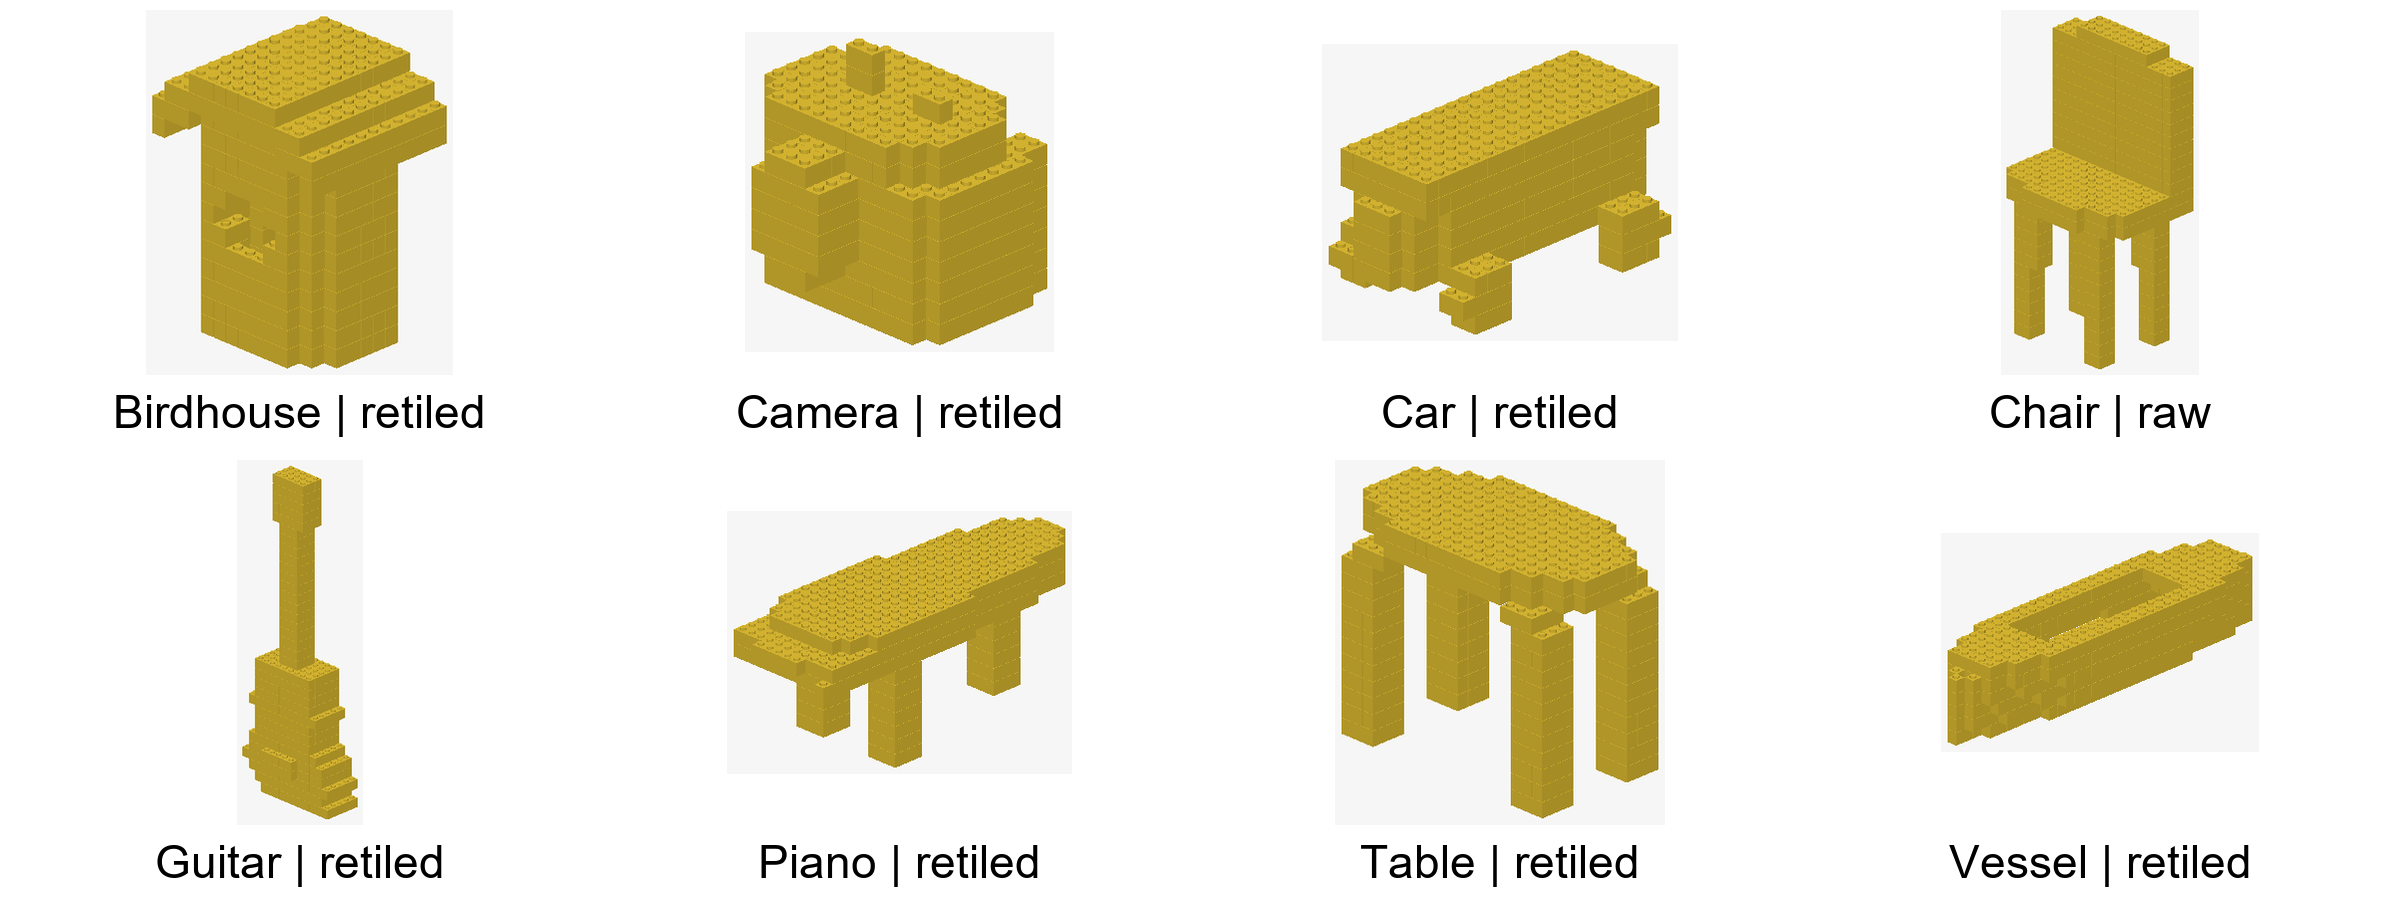
\includegraphics[width=\textwidth]{figures/generated_gallery_en.png}
\caption{BrickForma outputs from the earlier 114-prompt comparison. The chair is raw and the remaining examples are retiled.}
\end{figure*}
